\documentclass[12pt]{report}
\usepackage{verbatim}
\usepackage{fullpage}
\usepackage{etoolbox}
\usepackage{lipsum}
\usepackage{graphicx}
\usepackage{hyperref}
\usepackage{titlesec}
\usepackage{pdftexcmds}
\usepackage{minted}
\usepackage[utf8]{inputenc}
\usepackage{mathtools}


\graphicspath{ {res/} }
\setcounter{secnumdepth}{4}
\titleformat{\paragraph}
{\normalfont\normalsize\bfseries}{\theparagraph}{1em}{}
\titlespacing*{\paragraph}
{0pt}{3.25ex plus 1ex minus .2ex}{1.5ex plus .2ex}

\newcommand{\HRule}{\rule{\linewidth}{0.5mm}}
\renewcommand\emph{\textbf}
\renewcommand{\baselinestretch}{1.1}

\begin{document}
    \begin{titlepage}

        \center

        \textsc{\LARGE Universita' degli Studi di Messina}\\[0.1cm]
        \textsc{\Large Dipartimento di Matematica e Informatica}\\[0.5cm]
        \textsc{\Large Progetto Sistemi Operativi}\\[0.5cm]

        \HRule \\[0.4cm]
        { \huge \bfseries AllocSim}\\[0.1cm]

        {\large 24 Giugno 2015}
        \HRule \\[1.5cm]

        \begin{minipage}{0.4\textwidth}
        \begin{flushleft} \large
        \emph{Autore:}\\
        Vittorio \textsc{Romeo}
        \end{flushleft}
        \end{minipage}
        ~
        \begin{minipage}{0.4\textwidth}
        \begin{flushright} \large
        \emph{Professoressa:} \\
        Santa \textsc{Agreste}

        \end{flushright}
        \end{minipage}\\[4cm]

        \vfill

        \begin{minipage}{\linewidth}
            \centering
            \begin{minipage}{0.35\linewidth}
                \begin{figure}[H]
                    \center
                    
\includegraphics[width=2cm, height=2cm]{logovee}

                    \url{http://vittorioromeo.info}
                \end{figure}
            \end{minipage}
            \hspace{0.27\linewidth}
            \begin{minipage}{0.35\linewidth}
                \begin{figure}[H]
                    \center
                    
\includegraphics[width=2cm, height=2cm]{logounime}

                    \url{http://unime.it}
                \end{figure}
            \end{minipage}
        \end{minipage}\\[3cm]
    \end{titlepage}

    \pagenumbering{gobble}
    \newcommand{\atoc}[1]{\addtocontents{toc}{#1\par}}
    \renewcommand{\thesection}{\arabic{section}.}
    \tableofcontents
    \newpage
    \pagenumbering{arabic}

    \section{Richiesta}
        Si richiede l’implementazione di un applicativo che simuli tre delle tecniche usate per eseguire l’allocazione della memoria utilizzando una free-list: \emph{first-fit}, \emph{best-fit} e \emph{worst-fit}. 

        L’applicativo deve prevedere una situazione iniziale (randomica) della memoria e confrontare il risultato finale ottenuto dalle tre tecniche. 

        Supponendo che ogni confronto costi una unitò, si analizzino le differenze in termini di costo e in termini di frammentazione esterna.         

        L’applicativo deve effettuare delle simulazioni al fine di esaminare il diverso comportamento delle tre tecniche mostrando ad ogni simulazione lo stato del sistema sia a video che su file di log.

        L’applicativo deve essere sviluppato in \emph{Python}.

    \section{Algoritmi di allocazione}
        AllocSim implementa i seguenti algoritmi di allocazione dei processi.

        \begin{itemize}
            \item \emph{First-fit}: l'allocatore sceglierà il primo blocco abbastanza grande da poter contenere il processo.
            \item \emph{Next-fit}: l'allocatore sceglierà il primo blocco (a partire dalla posizione dell'allocazione precedente) abbastanza grande da poter contenere il processo.
            \item \emph{Best-fit (naive)}: l'allocatore scorrerà tutti i blocchi ed allocherà il processo in quello più piccolo che può contenerlo.
            \item \emph{Worst-fit (naive)}: l'allocatore scorrerà tutti i blocchi ed allocherà il processo in quello più grande.
            \item \emph{Best-fit (sorted list)}: l'allocatore terrà traccia dei blocchi in una lista ordinata per la loro grandezza. Partendo dall'inizio della lista sceglierà il primo blocco non occupato che può contenere il processo.
            \item \emph{Worst-fit (sorted list)}: l'allocatore terrà traccia dei blocchi in una lista ordinata per la loro grandezza. Partendo dalla fine della lista sceglierà il primo blocco non occupato che può contenere il processo.
        \end{itemize}        

    \section{Design ed implementazione}
        L'applicazione è stata implementata utilizzando il linguaggio di programmazione \emph{Python 2.6}.

        L'architettura dell'applicazione è stata designata utilizzando \emph{principi OOP} (Object-Oriented Programming) e massimizzando la riusabilità delle classi.

        Nella lista seguente sono riportati gli elementi che compongono l'architettura e il modo in cui sono relazionati:

        \begin{itemize}
            \item \emph{Blocco di memoria}: classe Python \mintinline{python}{Block} - rappresenta porzione dell'area di memoria presente nell'\emph{Allocatore}. Può essere \emph{occupato} o \emph{libero}, ha un \emph{byte di inizio} ed un \emph{byte di fine}.

                \begin{minted}[mathescape, linenos, numbersep=5pt, gobble=2, frame=lines, framesep=2mm, fontsize=\footnotesize]{python}
    # Class representing a block of memory
    class Block:
        # Constructor
        def __init__(self, mAllocator, mStart, mEnd):
            # Allocator that owns the block
            self.allocator = mAllocator

            # Byte where the memory block begins
            self.start = mStart

            # Byte where the memory block ends
            self.end = mEnd

            # Is the memory block currently occupied?
            self.occupied = False

        # Returns the size of the memory block in bytes
        def getSize(self):
            return self.end - self.start
                \end{minted}

            \item \emph{Allocatore}: classe Python \mintinline{python}{Allocator} - rappresenta un'area di memoria contigua che può essere frammentata ed utilizzata per instanziare \emph{processi}. L'area di memoria viene divisa in \emph{blocchi}.  Contiene una lista di blocchi ordinata per posizione (in byte), una lista di blocchi ordinata per grandezza (utilizzata per implementare versioni degli algoritmi \emph{best-fit} e \emph{worst-fit} più efficienti), ed una lista di blocchi calcolata a runtime dei blocchi adiacenti liberi (\emph{boundary-tag}). 
            L'allocatore permette di \emph{dividere} un blocco in due in una specifica posizione, di \emph{occupare} o \emph{liberare} la memoria, e di \emph{unificare} i blocchi contigui liberi.

            \begin{minted}[mathescape, linenos, numbersep=5pt, gobble=2, frame=lines, framesep=2mm, fontsize=\footnotesize]{python}
    # Class representing a memory allocator
    class Allocator:
        # Constructor
        def __init__(self, mSize): ...

        # Restores the allocator to its original state
        def reset(self): ...

        # Return a tuple containing the block that includes the byte 'mX' and its index
        def getBlockAt(self, mX): ...

        # Inserts a block in the sorted list, in the correct position
        def insertSorted(self, mX): ...

        # Splits the memory owned by the allocator at the byte 'mX'
        # Returns a tuple containing the two halves in which the block was split and the
        # index of the first half
        def splitAt(self, mX): ...

        # Merges all adjacent unoccupied blocks
        def reclaim(self): ...

        # Free the memory in all the blocks, making them unoccupied
        def free(self): ...

        # Print an ASCII graph of the state of the allocator
        def printInfo(self): ...

        # Return a number representing the average fragmentation of the allocator
        def getFragmentation(self): ...

        # Execute an algorithm and print its result
        def executeAlgorithm(self, mAlgorithm, mX): ...

        # The "first fit" algorithm simply iterates over all blocks
        # until it finds a block which is suitable for the desired
        # memory allocation
        def insertFirstFit(self, mX): ...

        # The "next fit" algorithm uses the same logic as the "first fit" algorithm,
        # but starts looking for an unoccupied block at the last block index
        def insertNextFit(self, mX): ...

        # The "best fit" algorithm iterates over all available blocks
        # and selects the one that wastes less space for the memory allocation
        # This algorithm could be improved by keeping a separate list of memory blocks,
        # ordered by size
        def insertBestFitNaive(self, mX): ...


        # The "worst fit" algorithm iterates over all available blocks
        # and selects the one that wastes most space for the memory allocation
        # This algorithm could be improved by keeping a separate list of memory blocks,
        # ordered by size
        def insertWorstFitNaive(self, mX): ...

        # The "best fit" algorithm starts from the beginning of the sorted list
        def insertBestFitSL(self, mX): ...

        # The "worst fit" algorithm starts from the end of the sorted list
        def insertWorstFitSL(self, mX): ...
            \end{minted}


            L'allocatore contiene tutta la logica riguardante l'esecuzione degli \emph{algoritmi} richiesti, ed anche la logica per la generazione di un \emph{grafico ASCII} che rappresenta lo stato dell'area di memoria.
            \item \emph{Algorithmi}: contenuti nella classe Python \mintinline{python}{Allocator} - oltre agli algoritmi richiesti (\emph{first-fit}, \emph{best-fit}, \emph{worst-fit}), sono stati designati ed implementati anche i seguenti: \emph{next-fit}, \emph{best-fit} (con lista ordinata), e \emph{worst-fit} (con lista ordinata).
            Gli algoritmi agiscono sui \emph{blocchi}, liberi o occupati da \emph{processi}.


            \item \emph{Simulazione}: gestite da Python tramite le funzioni \mintinline{python}{runSimulations} and \mintinline{python}{simulate} - una simulazione, al suo inizio, genera una lista randomica di \emph{processi}, la quale viene testata in N \emph{sottosimulazioni}, le quali eseguono uno degli \emph{algoritmi} sulla medesima lista di processi, restituendo un \emph{set di risultati}.



            \item \emph{Sottosimulazione}: esegue un \emph{algoritmo} su un set di \emph{processi} generato randomicamente. Pulisce l'\emph{allocatore} dalle sottosimulazioni precedenti ed esegue calcoli statistici per verificare l'efficienza di un algoritmo, riportata in un \emph{set di risultati}.
            \item \emph{Processo}: classe Python \mintinline{python}{Process} - rappresenta un processo del sistema operativo utilizzato per le simulazioni automatiche. Ogni processo ha un \emph{tempo di entrata} (momento in cui il sistema prova ad allocare il processo), un \emph{tempo di esecuzione} (numero di unità di tempo necessarie al completamento del processo), un numero di \emph{byte richiesti} per l'esecuzione del processo (che saranno forniti, se possibile, attraverso l'allocazione di un \emph{blocco} libero). I processi randomicamente vengono generati all'inizio di una \emph{simulazione}.

            \begin{minted}[mathescape, linenos, numbersep=5pt, gobble=2, frame=lines, framesep=2mm, fontsize=\footnotesize]{python}
    # Class representing a single process
    class Process:
        # Constructor
        def __init__(self, mID, mStart, mRequired, mMem):
            # Process ID
            self.id = mID

            # Execution start time
            self.start = mStart

            # Time required for execution
            self.required = mRequired

            # Memory required for execution
            self.size = mMem

            # Block being occupied by the process
            self.block = None

        # Returns 'True' if the process has ended
        def finished(self):
            return self.required <= 0
            \end{minted}

            \item \emph{Set di risultati}: instanziato e stampato alla fine di una \emph{simulazione}. Contiene informazioni riguardo il \emph{numero di comparazioni}, \emph{frammentazione media} e \emph{punteggio totale} di ogni \emph{algoritmo} testato durante la simulazione. Minore il punteggio, più efficiente l'algoritmo.
        \end{itemize}

        L'applicativo può essere eseguito in due modalità: \emph{modalità manuale} e \emph{modalità automatica}.

        \begin{itemize}
            \item \emph{Modalità manuale}: gestita dalla funzione Python \mintinline{python}{mainManual} - questa modalità permette all'utente di interagire manualmente con l'\emph{allocatore}, eseguendo allocazioni singole e visualizzando tramite un \emph{grafico ASCII} il loro risultato.

            \item \emph{Modalità automatica}: gestita dalla funzione Python \mintinline{python}{mainAutomatica} - genera N simulazioni (valore passato da linea di comando, come primo parametro) e le esegue, scrivendo a video e su log i loro risultati. 
        \end{itemize}

    \section{Statistiche}
        Le statistiche effettuate dall'applicativo sono le seguenti:

        \begin{itemize}
            \item \emph{Confronti effettuati}: per verificare l'efficienza di un algoritmo rispetto ad un altro verrà conteggiato il numero dei confronti effettuati nella ricerca di un blocco adatto ad un processo.
            \item \emph{Frammentazione esterna media}: ogni iterazione di una simulazione verrà conservata ed accumulata la frammentazione esterna corrente. Alla fine della simulazione la frammentazione accumulata verrà divisa per il numero di iterazioni e mostrata all'utente.

            Durante una singola iterazione la frammentazione media viene calcolata con la formula seguente:

            $ externalFragmentation = 1.0 - \frac{biggestFreeBlockSize}{totalFreeMemory} $

        \end{itemize}

    \section{Diagrammi UML}

        \subsection{Class diagram}

            Viene qui riportato il \emph{class diagram UML} delle classi contenute nel progetto.
            Il diagramma è stato realizzato automaticamente dall'applicazione \mintinline{python}{pyreverse}.

            \begin{figure}[H]
                \caption{Diagramma UML delle classi.}
                \centering
                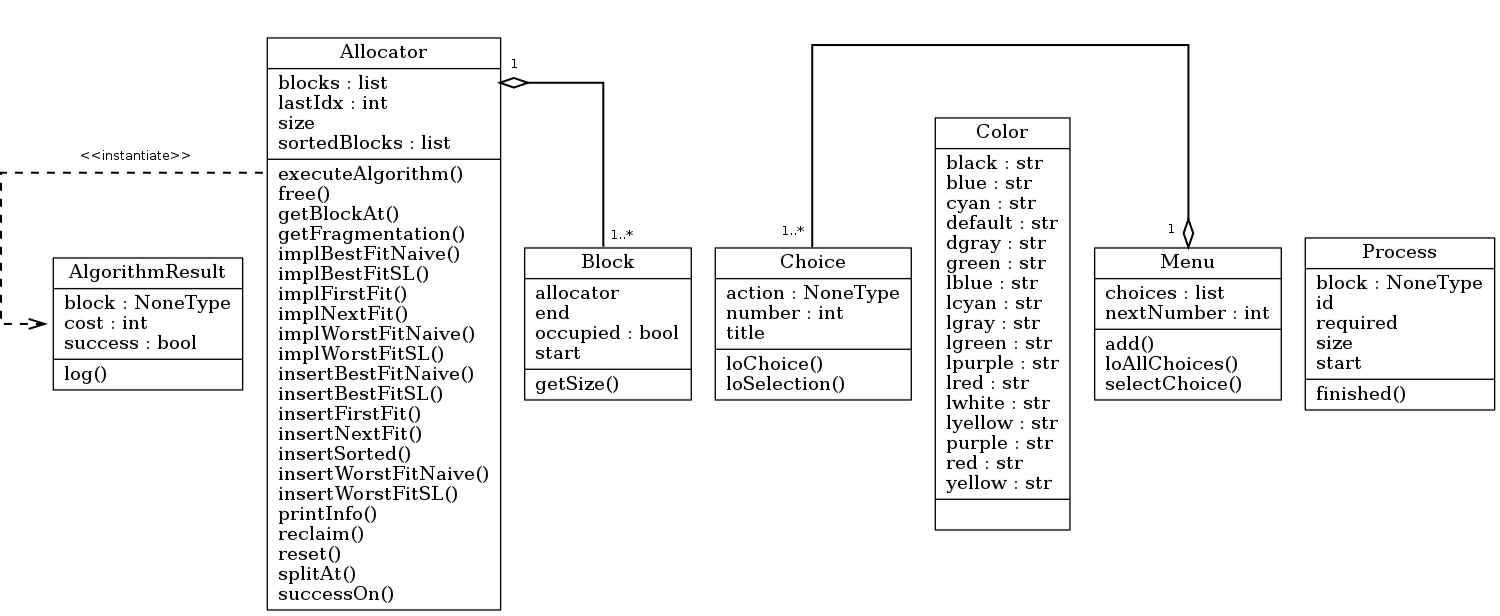
\includegraphics[width=1\textwidth]{diatemp}
            \end{figure}

        \subsection{Activity diagram}

            Sono riportati a seguire due \emph{activity diagram}, che mostrano la funzionalità dell'applicativo al suo avvio e il funzionamento dell'algoritmo best-fit.

            \begin{figure}[H]
                \caption{Diagramma: esecuzione applicativo.}
                \centering
                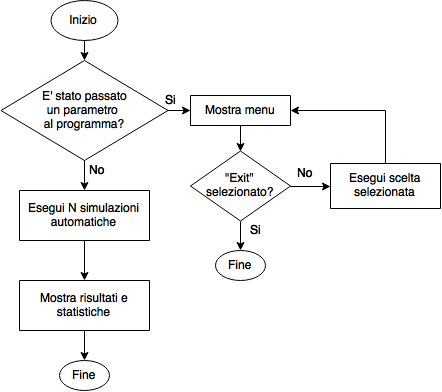
\includegraphics[width=1\textwidth]{dia0}
            \end{figure}

            \begin{figure}[H]
                \caption{Diagramma: algoritmo best fit.}
                \centering
                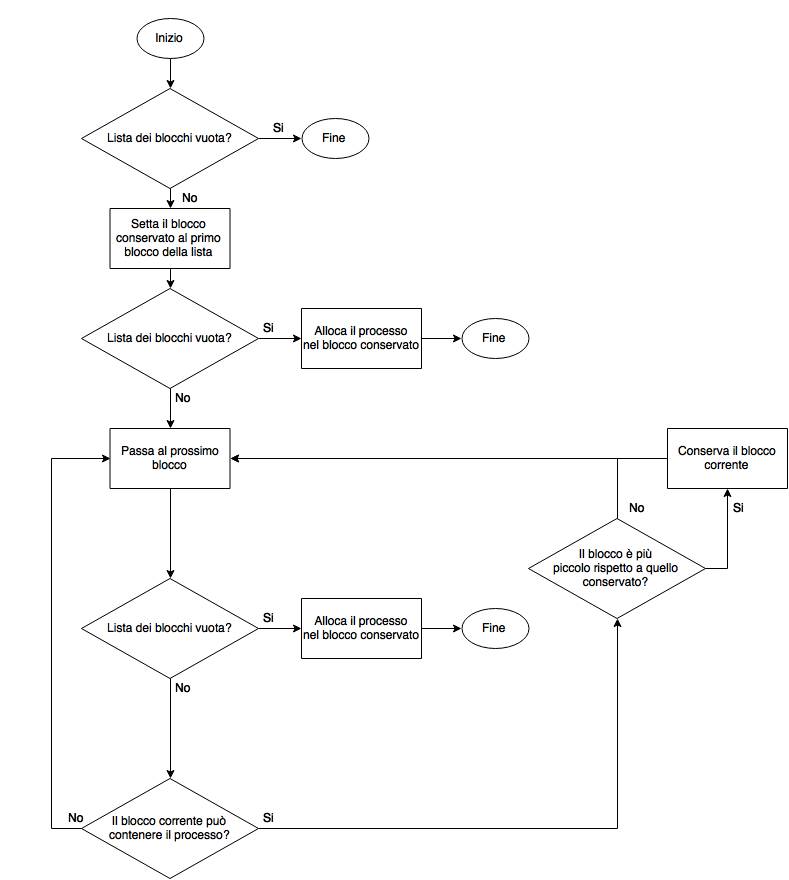
\includegraphics[width=1\textwidth]{dia1}
            \end{figure}


    \section{Manuale d'uso}

        L'applicazione è molto \emph{user-friendly}: semplice da usare e robusta. Gli input forniti dall'utente vengono controllati, ed in caso di input non validi l'utente può ritentare senza causare errori o crash.

        \subsection{Modalità manuale}

            Per avviare l'applicazione in \emph{modalità manuale} è sufficiente lanciarla da linea di comando senza parametri:

            \begin{minted}[mathescape, linenos, numbersep=5pt, gobble=2, frame=lines, framesep=2mm, fontsize=\footnotesize]{bash}
    ./project.py
            \end{minted}

            Dopo aver avviato il programma, l'utente vedrà il seguente menù:

            \begin{figure}[H]
                \caption{Screenshot: menù modalità manuale.}
                \centering
                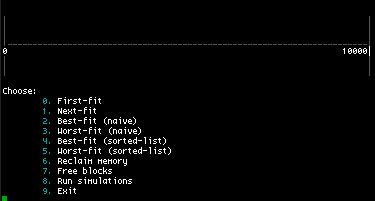
\includegraphics[width=0.6\textwidth]{scr1}
            \end{figure}

            L'utente potrà scegliere tra le varie funzioni dell'allocatore e visualizzare su schermo in maniera grafica i loro risultati.

        \subsection{Modalità automatica}

            Per avviare l'applicazione in \emph{modalità automatica} è sufficiente lanciarla da linea di comando con il numero di simulazioni desiderato:

            \begin{minted}[mathescape, linenos, numbersep=5pt, gobble=2, frame=lines, framesep=2mm, fontsize=\footnotesize]{bash}
    # Esempio (3 simulazioni) 
    ./project.py 3
            \end{minted}

            Dopo aver avviato il programma, le simulazioni partiranno automaticamente ed il loro funzionamento sarà mostrato sia a video che su log.

            \begin{figure}[H]
                \caption{Screenshot: modalità automatica.}
                \centering
                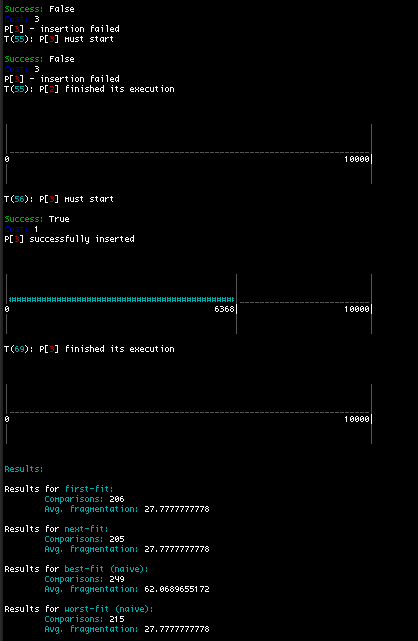
\includegraphics[width=0.6\textwidth]{scr2}
            \end{figure}

        \section{Risultati ottenuti}

            Avendo eseguito 1000 simulazioni ripetutamente ed avendo calcolato la media sui dati statistici restituiti da esse, notiamo che i valori riportati sono in linea con quelli comunemente aspettati per gli algoritmi scelti.

            \begin{minted}[mathescape, linenos, numbersep=5pt, gobble=2, frame=lines, framesep=2mm, fontsize=\footnotesize]{python}
    TOTAL Results for first-fit:
        Avg. comparisons: 419
        Avg. fragmentation: 37.0976293895

    TOTAL Results for next-fit:
        Avg. comparisons: 405
        Avg. fragmentation: 37.227405137

    TOTAL Results for best-fit (naive):
        Avg. comparisons: 419
        Avg. fragmentation: 35.3508336604

    TOTAL Results for worst-fit (naive):
        Avg. comparisons: 442
        Avg. fragmentation: 37.4901873478

    TOTAL Results for best-fit (sorted list):
        Avg. comparisons: 432
        Avg. fragmentation: 35.7433916187

    TOTAL Results for worst-fit (sorted list):
        Avg. comparisons: 416
        Avg. fragmentation: 37.0976293895
            \end{minted}

            I risultati sono stati calcolati simulando l'entrata ed uscita continua di processi di dimensioni randomiche e durata randomica.

            E' possibile notare che, utilizzando questo tipo di simulazione:

            \begin{itemize}
                \item il numero medio di comparazioni e frammentazione su tutte le 1000 simulazioni varia poco in base all'algoritmo. Questo è dovuto alla grandezza e durata randomica dei processi: è a volte possibile che un processo occupi l'intero allocatore per più unità di tempo o che molti processi piccoli e rapidi escano ed entrino continuamente.
                \item gli algoritmi \emph{first-fit} e \emph{next-fit} hanno risultati estremamente simili. Il \emph{next-fit}, tuttavia, ha in media un numero minore di comparazioni in quanto i blocchi allocati in precedenza vengono subito saltati grazie all'indice conservato che punta al blocco dell'ultimo allocazione.
                \item l'algoritmo \emph{best-fit} (sia naive che con sorted-list) ha sempre \emph{frammentazione esterna minore} rispetto all'algoritmo \emph{worst-fit} (sia naive che sorted-list). Il numero di comparazioni tra i due non è legato alla scelta dell'algoritmo ma alla generazione randomica dei processi - il \emph{worst-fit} può avere meno comparazioni del \emph{best-fit} e viceversa.
            \end{itemize}

\end{document}
